% Created 2019-01-22 Di 09:07
% Intended LaTeX compiler: pdflatex
\documentclass[10pt, a4paper]{scrartcl}
\usepackage[utf8]{inputenc}
\usepackage[T1]{fontenc}
\usepackage{graphicx}
\usepackage{grffile}
\usepackage{longtable}
\usepackage{wrapfig}
\usepackage{rotating}
\usepackage[normalem]{ulem}
\usepackage{amsmath}
\usepackage{textcomp}
\usepackage{amssymb}
\usepackage{capt-of}
\usepackage{hyperref}
\usepackage[ngerman, germanb]{babel}
\usepackage[a4paper,margin=2.54cm]{geometry}
\author{Stefan Schuh\thanks{stefan.schuh@uni-graz.at}}
\date{2019-01-22}
\title{Dokumentation für BearbeiterInnen}
\hypersetup{
 pdfauthor={Stefan Schuh},
 pdftitle={Dokumentation für BearbeiterInnen},
 pdfkeywords={},
 pdfsubject={},
 pdfcreator={Emacs 25.2.2 (Org mode 9.2)}, 
 pdflang={Germanb}}
\begin{document}

\maketitle
\tableofcontents

\section{Allgemeines}
\label{sec:org9284342}
In Alma gibt es Datensätze (größenteils Zeitschriften und Reihen), an denen
für jedes Exemplar ein Holding vorhanden ist, obwohl eigentlich die ganzen
Exemplare an einem oder wenigen Holdings hängen sollten. Meistens ist das
der Fall, weil in Aleph kein Holding an diesem Titel vorhanden war. Nachdem
jedes Exemplar eine andere Signatur hatte (\texttt{I 12345/1}, \texttt{I 12345/2}, usw.),
wurde bei der Migration für jedes einzelne ein eigenes Holding gebildet. Das
wollen wir nun bereinigen.

Nachdem das bei mehr als 40.000 Exemplaren intellektuell nicht zu leisten
ist, gibt es zu diesem Zweck ein kleines Programm, das Sie dabei
unterstützt.

Der Ablauf für Sie schaut folgendermaßen aus:

\begin{itemize}
\item Zielholding identifizieren/erstellen
\item Programm aufrufen
\item Falls mehrere Grundsignaturen vorhanden (z. B. "`N.F."'), mit nächster
Grundsignatur wiederholen, bis alles Exemplare richtig hängen
\item Falls noch nicht geschehen, die Informationen in den Holdings ergänzen,
die noch fehlen
\end{itemize}

\subsection{Zuordnung von Exemplaren an das Zielholding}
\label{sec:org47f1899}
Im Zuge der Verarbeitung werden alle Holdings auf Übereinstimmungen mit dem
Zielholding geprüft. Wenn die richtigen Werte übereinstimmen, werden die
Exemplare von diesen Holdings ans Zielholding gehängt und das dann
überflüssige Holding gelöscht.

Die Überprüfung, ob ein Exemplar sich zum Umhängen qualifiziert, läuft
über das Feld \texttt{852} im Holding:

\begin{itemize}
\item \texttt{\$\$b} muss übereinstimmen
\item \texttt{\$\$c} muss übereinstimmen
\item \texttt{\$\$h} genauso \emph{beginnen} wie \texttt{\$\$h} im Zielholding
\end{itemize}


\subsubsection{Ein paar Beispiele}
\label{sec:org69fc0e4}
Zielholding: \texttt{852 81 \$\$b BDEPO \$\$c DHB \$\$h II 47550}

\begin{center}
\begin{tabular}{lll}
Informationen im Ausgangshol & Match & Kommentar\\
\hline
\texttt{\$\$b BHB \$\$c MAG \$\$h II 47550/1} & Nein & \texttt{\$\$b} und \texttt{\$\$c} stimmen nicht überein\\
\texttt{\$\$b BDEPO \$\$c DHB \$\$h II 47550/N.F.2} & Ja & \texttt{\$\$b} und \texttt{\$\$c} stimmen überein\\
 &  & \texttt{\$\$h} beginnt wie \texttt{\$\$h} im Zielholding\\
\texttt{\$\$b BDEPO \$\$c DHB \$\$h II 47550/3} & Ja & \\
\texttt{\$\$b BDEPO \$\$c DHBMA \$\$h 47550/1} & Nein & \texttt{\$\$c} stimmt nicht überein\\
\end{tabular}
\end{center}

Wir sehen, dass sowohl \texttt{II 47550/3} als auch \texttt{II 47550/N.F.2} der
Grundsignatur zugeordnet werden, obwohl hier eigentlich zwei Holdings
angelegt werden müssten. Das ist technisch nicht anders möglich. Daher
ist die Reihenfolge, in der diese Exemplare bearbeitet werden
entscheidend. Mehr dazu im Abschnitt \ref{sec:org2eb550b}.



\subsubsection{Die Grundsignatur}
\label{sec:org9ba1d80}
Um ein Zielholding zu identifizieren bzw. zu erstellen, müssen wir klären,
was wir in diesem Zusammenhang unter dem Begriff \emph{Grundsignatur} verstehen:

Unter \textbf{Grundsignatur} verstehen wir den Teil einer Signatur, der \emph{mehreren
Exemplaren einer Zählfolge gemeinsam} ist. Z. B. \texttt{I 156715}, aber auch \texttt{I
        156715/N.F.} oder \texttt{I 156715/3.Ser.}. Diese Unterscheidung ist wichtig, weil
die Zuordnung der Exemplare an ein Zielholding unter anderem dadurch
passiert, dass die Signatur im zu bereinigenden Holding gleich anfängt, wie
die im Zielholding.
\section{Arbeitsablauf}
\label{sec:org81ce472}
\subsection{MMS-ID des bibliografischen Datensatzes ermitteln}
\label{sec:org9ca9c11}
Damit das Programm arbeiten kann brauchen wir die \emph{lokale} MMS-ID des
Titeldatensatzes und die MMS-ID des Zielholdings. Am einfachsten ist es,
wenn man sich diese Nummern irgendwo zwischenspeichert (im Editor z. B.), um
sie dann in die Eingabefelder zu kopieren.

Wie kommt man zur lokalen MMS-ID? Die lokale MMS-ID ist die, die mit 3339
endet (im Gegensatz zu 3331 in der NZ). Am einfachsten kommt man zu dieser
in der Datensatz-Ansicht (d. h. wenn man beim Suchergebnis auf den Titel
klickt):

\begin{center}
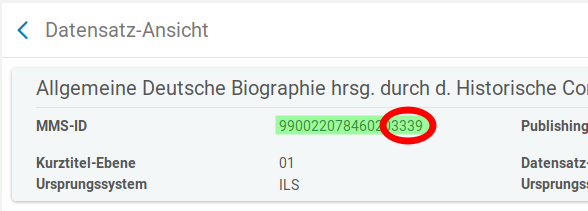
\includegraphics[width=.9\linewidth]{/home/schuhs/projects/multi-hol/doc/pic/mmsid_bib.png}
\end{center}

Diese Nummer muss mit \texttt{99} anfangen und mit \texttt{3339} aufhören. Öffnen Sie
den Texteditor -- einfach Windows-Taste drücken und "`Editor"' eingeben: 

\begin{center}
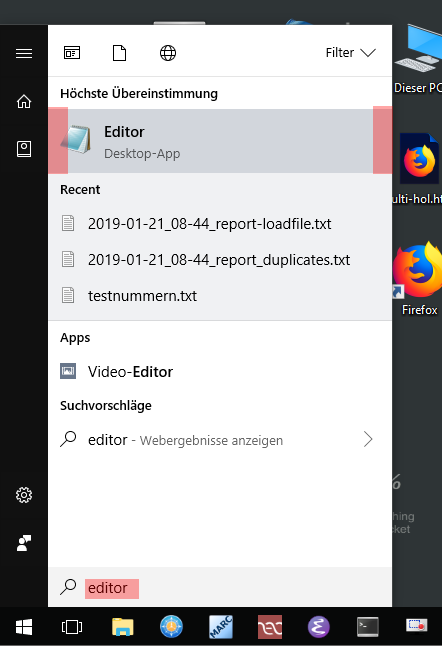
\includegraphics[width=.9\linewidth]{/home/schuhs/projects/multi-hol/doc/pic/start_edit.png}
\end{center}

Kopieren Sie die Nummer hinein.
\subsection{Das Ziel-Holding identifizieren/anlegen}
\label{sec:org2c82a7c}
In den allermeisten Fällen müssen Sie das Zielholding neu anlegen. Das
geht aber recht schnell:

\begin{enumerate}
\item Suchen Sie ein beliebiges Holding am gleichen Standort, mit der
Grundsignatur, die Sie brauchen und öffnen Sie dieses im Metadateneditor
zum bearbeiten
\item Klicken Sie auf [Datei -> Duplizieren]
\item Im duplizierten Holding (erkennbar am ausgegrauten Symbol) löschen Sie
den hinteren Teil der Signatur, sodass nur die Grundsignatur übrig bleibt:

\begin{center}
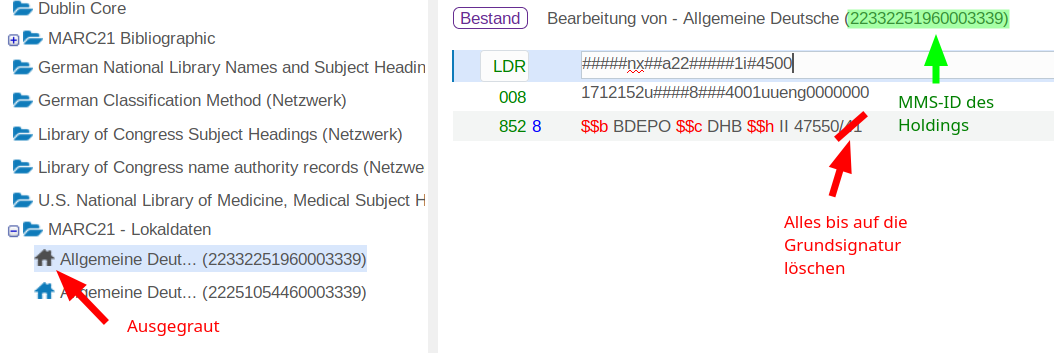
\includegraphics[width=.9\linewidth]{/home/schuhs/projects/multi-hol/doc/pic/dupliziertes_hol.png}
\end{center}
\item Klicken sie auf \texttt{Speichern}
\item Kopieren Sie die MMS-ID des Holdings (siehe den grünen Pfeil im Bild bei
Punkt 3) auch in den Editor. Die MMS-ID eines Holdings beginnt immer
mit \texttt{22} und endet mit \texttt{3339}. Im Bild sehen Sie das Editorfenster mit
der MMS-ID des Bibsatzes in der ersten und der des Holdings in der
zweiten Zeile.

\begin{center}
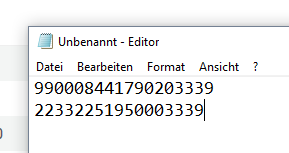
\includegraphics[width=.9\linewidth]{/home/schuhs/projects/multi-hol/doc/pic/mmsid_editor.png}
\end{center}
\end{enumerate}
\subsection{Das Programm ausführen}
\label{sec:orge92c025}
Jetzt, wo Sie das Zielholding angelegt haben und die MMS-IDs vom
bibliografischen Datensatz und vom Holding in den Editor kopiert haben,
können Sie das Programm ausführen. Wo es genau liegt, haben Sie
normalerweise bei der Einschulung erfahren, wahrscheinlich haben Sie auch
eine Verknüpfung auf Ihrem Desktop. Machen Sie einen Doppelklick auf das
Programm und nach ein paar Sekunden kommt ein Eingabefenster:

\begin{center}
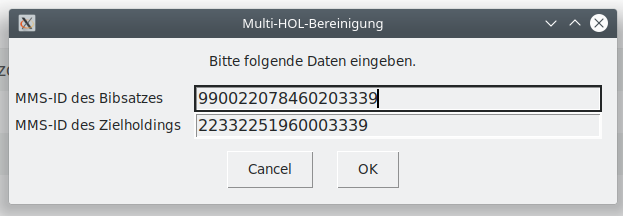
\includegraphics[width=.9\linewidth]{/home/schuhs/projects/multi-hol/doc/pic/eingabefenster.png}
\end{center}

Fügen Sie die jeweiligen Nummern in die entsprechenden Felder ein und
klicken Sie auf "`OK"'.

Im schwarzen Fenster das sich auch mit dem Programm geöffnet hat, sehen
Sie den Fortschritt der des Programms. Wenn es fertig ist, sehen Sie die
Zeilen

\begin{center}
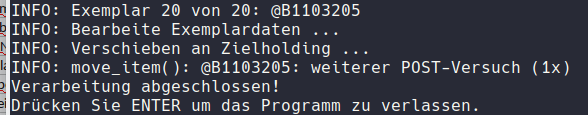
\includegraphics[width=.9\linewidth]{/home/schuhs/projects/multi-hol/doc/pic/verarbeitung_abgeschlossen.png}
\end{center}

Wenn Sie \texttt{ENTER} drücken, schließt sich das Fenster und das Progamm ist beendet.
\subsection{Die Zusammenfassende Bestandsangabe, etc. in Zielholding eintragen}
\label{sec:orgbdbfbe3}
Nach Ausführung des Programms sollte es am Datensatz für Ihre Signatur nur
noch ein Holding geben, an dem alle Exemplare hängen. Überprüfen Sie, was
da ist und machen Sie eine entsprechende zusammenfassende Bestandsangabe
im Holding.

Es ist empfehlenswert, diesen Schritt am Schluss zu machen, weil es sein
kann, dass die Bearbeitung mit weiteren Grundsignaturen ("`N.F."', etc.;
siehe \ref{sec:org2eb550b})
wiederholt werden muss. Erst wenn alle Exemplare richtig hängen, lassen
sich die Angaben in den Holdings korrekt machen.
\section{Spezialfälle}
\label{sec:orgf4176c4}
\subsection{Mehrere Grundsignaturen an einem bibliografischen Datensatz}
\label{sec:org2eb550b}
Manchmal ist es notwendig, die Exemplare an einem bibliografischen
Datensatz auf mehrere Holdings aufzuteilen. Das kommt dann vor, wenn es
mehrere Zählfolgen gibt. Jede dieser Zählfolgen hatte eine eigene \hyperref[sec:org9ba1d80]{Grundsignatur}, 
für die jeweils ein eigenes Holding angelegt werden muss.

Wenn wir uns das Beispiel von \ref{sec:org69fc0e4} noch einmal ansehen,
bemerken wir, dass die Signaturen \texttt{II 47550/3} und \texttt{II 47550/N.F.2} beide
dem gleichen Zielholding zugeordnet werden. Nachdem der Anfang der
Signatur übereinstimmt, lässt sich das nicht verhindern. Im Endeffekt
funktioniert das Ganze aber trotzdem, wenn wir die Signaturen in der richtigen
Reihenfolge, nämlich beginnend mit der kürzesten Signatur, abarbeiten.

Würden wir diese Reihenfolge nicht einhalten, d. h. z. B. zuerst \texttt{II
      47550/N.F.} und erst dann \texttt{II 47550} bearbeiten, würden beim zweiten Lauf
die Exemplare alle von \texttt{II 47550/N.F.} wegwandern und sich an \texttt{II 47550}
hängen (weil ihre Signatur ja auch mit \texttt{II 47550} beginnt). Umgekehrt
passiert das nicht, weil z. B. \texttt{II 47550/23} ja nicht mit \texttt{II 47550/N.F.}
anfängt.

Das kling komplizierter, als es in der Praxis ist:

\begin{enumerate}
\item Zuerst das Zielholding für die \emph{kürzeste} Signatur anlegen und das
Programm ausführen. Damit hängen sich \emph{alle} Exemplare an dieses
Holding.
\item Danach das Zielholding für die nächste Signatur (z. B. \texttt{II 47550/N.F.})
anlegen und das Programm ausführen. Damit wandern die Exemplare der
Neuen Folge vom ersten Zielholding an das richtige. An diesem Punkt ist
die Reihenfolge nicht mehr wichtig, d. h. es ist egal ob man jetzt mit
der neuen Folge oder der 3. Serie weitermacht.
\item Diesen Vorgang mit allen notwendigen Grundsignaturen wiederholen, bis alle
Exemplare beim richtigen Holding sind.
\end{enumerate}
\subsubsection{Ein Beispiel für mehrere Signaturen}
\label{sec:orgbf0db5f}
Hier ein Screenshot der Holdings-Liste vor der Bearbeitung, an jedem HOL
gibt es genau ein Exemplar:

\begin{center}
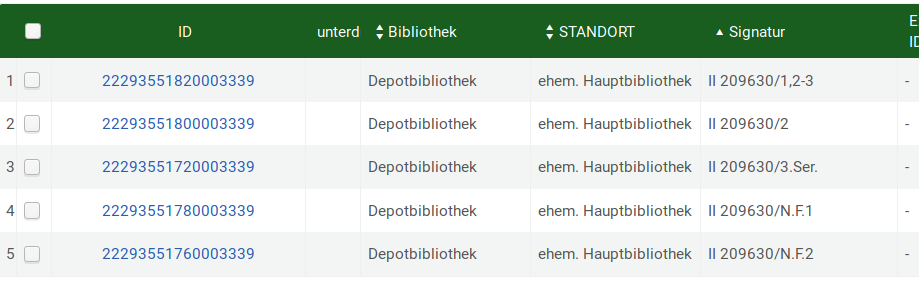
\includegraphics[width=.9\linewidth]{/home/schuhs/projects/multi-hol/doc/pic/holdings_vorher.png}
\end{center}

Nachdem wir ein Holding für \texttt{II 209630} angelegt und unser Programm haben
laufen lassen, gibt es nur noch ein Holding (dafür mit 5 Exemplaren):
\begin{center}
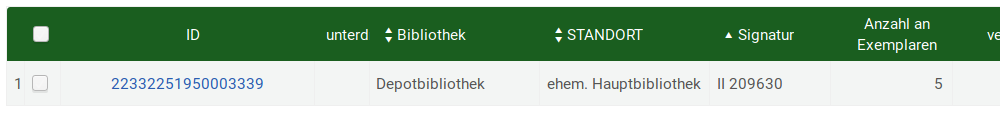
\includegraphics[width=.9\linewidth]{/home/schuhs/projects/multi-hol/doc/pic/holding_nachher.png}
\end{center}

Wenn wir die Exemplare dieses Holdings anzeigen lassen, sehen wir in der
alternativen Signatur die einzelnen Signaturen für die Exmplare. Auch die
neue Folge und die 3. Serie sind hier vertreten:

\begin{center}
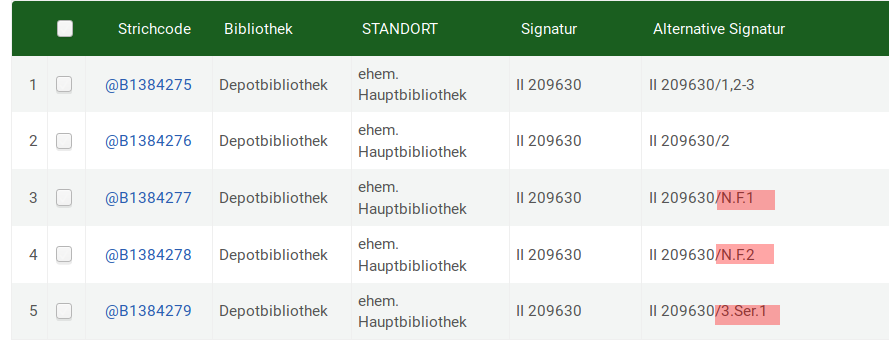
\includegraphics[width=.9\linewidth]{/home/schuhs/projects/multi-hol/doc/pic/exemplare_nachher1.png}
\end{center}

Also legen wir ein weiteres Holding mit der Signatur \texttt{II 209630/N.F.} an
und führen das Programm noch einmal aus. Wieder die gleiche MMS-ID für den
Bibsatz, aber die MMS-ID für das gerade angelegte neue Holding. Danach
gibt es zwei Holdings:

\begin{center}
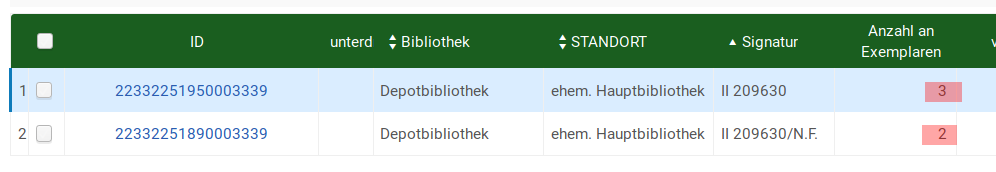
\includegraphics[width=.9\linewidth]{/home/schuhs/projects/multi-hol/doc/pic/holdings_nachher2.png}
\end{center}

Wir sehen, dass bei \texttt{II 209630} nur noch drei Exemplare sind, die anderen
beiden sind zu \texttt{II 209630/N.F.} gewandert. Nun fehlt uns noch das eine
Exemplar für die 3. Serie. Also legen wir noch ein Holding mit \texttt{II
        209630/3.Ser.} an und lassen das Programm noch einmal laufen. Dann gibt es
drei Holdings:

\begin{center}
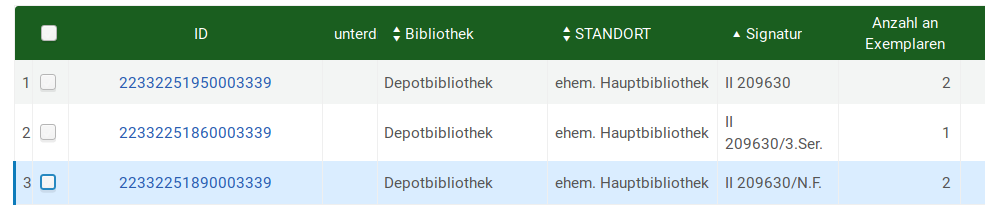
\includegraphics[width=.9\linewidth]{/home/schuhs/projects/multi-hol/doc/pic/holdings_nachher3.png}
\end{center}

Wenn wir alle Exemplare anzeigen und dort die Signatur und die alternative
Signatur ansehen, sehen wir, dass jetzt alles richtig hängt:

\begin{center}
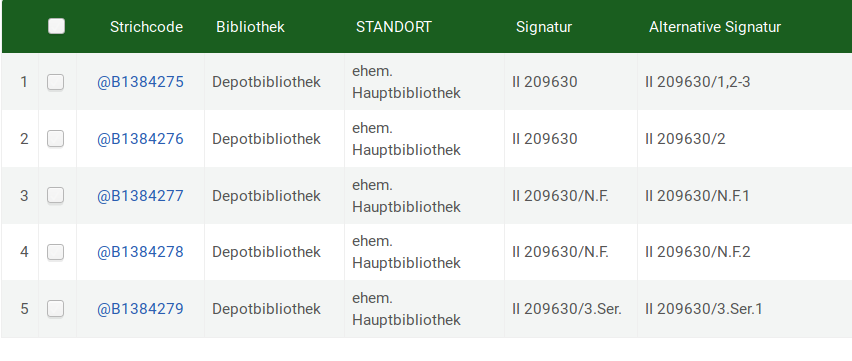
\includegraphics[width=.9\linewidth]{/home/schuhs/projects/multi-hol/doc/pic/exemplare_nachher2.png}
\end{center}

Nun können wir die restlichen Daten in den Holdings nachtragen:

Bei \texttt{II 209630}:

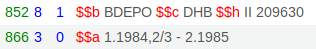
\includegraphics[width=5cm]{/home/schuhs/projects/multi-hol/doc/pic/bestand1.png}

Bei \texttt{II 209630/N.F.}:

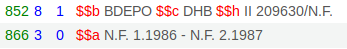
\includegraphics[width=5cm]{/home/schuhs/projects/multi-hol/doc/pic/bestand2.png}

Bei \texttt{II 209630/3.Ser.}:

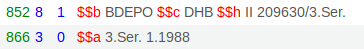
\includegraphics[width=5cm]{/home/schuhs/projects/multi-hol/doc/pic/bestand3.png}
\subsection{Fehlermeldungen}
\label{sec:org7eb7aab}
Wenn alles reibungslos funktioniert sehen sie in dem Terminalfenster, das
sich mit dem Programm öffnet, diverse Informationen vorbeiziehen. Was
diese genau bedeuten, muss Sie nicht weiter interessieren. Sie sehen das
nur, damit Sie wissen, dass das Programm etwas tut -- es kann nämlich
recht lange dauern, wenn viele Exemplare umgehängt werden. Führen Sie das
Programm also lieber nicht aus, kurz bevor Sie nachhause gehen wollen. ;-)

Normalerweise beginnt jede einzelne Zeile mit \texttt{INFO:}. Wenn das der Fall
ist, ist alles ok. Es kann aber auch sein, dass einmal eine Zeile mit
\texttt{ERROR:} beginnt. Dann hat etwas nicht funktioniert. Üblicherweise
passiert das, wenn ein Exmplar entlehnt ist, oder eine Bestellung mit dem
Exemplar oder dem Holding verbunden ist.

Das ist in den meisten Fällen kein Grund zur Besorgnis: Das Programm läuft
weiter und lässt das betroffene Holding samt Item in Ruhe. Allerdings
müssen Sie dieses dann manuell bereinigen. Das heißt, wenn eine Bestellung
damit verbunden ist, diese entsprechend bearbeiten, nämlich mit dem
Zielholding verbinden. Wenn das Exemplar entlehnt ist, müssen Sie eh
warten, bis es zurück ist und können es dann umhängen.

Hier zwei Beispiele für typische Fehlermeldungen:

\textbf{Bestellung vorhanden:}

\phantomsection
\label{org4a66c0f}
\begin{verbatim}
ERROR: move_item(): löschen fehlgeschlagen bei @B1103200. {"errorsExist":true,
"errorList":{"error":[{"errorCode":"401849","errorMessage":"Item delete errors:
There is a PO line POL-13073 linked to this item @B1103200. Please handle the 
order (using the PO line pages) before withdrawing this item / these items. \n",
"trackingId":"E01-2101110719-OYNS8-AWAE1622782160"}]},"result":null}
\end{verbatim}

\textbf{Exemplar entlehnt:}

\begin{verbatim}
ERROR: move_item(): löschen fehlgeschlagen bei @B1303276. {"errorsExist":true,
"errorList":{"error":[{"errorCode":"401849","errorMessage":"Item delete errors:
There are loans registered for item @B1303276. Please handle the loans before deleting
this item / these items. \n","trackingId":"E01-2201074327-ZSZQY-AWAE1622782160"}]},
"result":null}
\end{verbatim}

Bei solchen Fehlermeldungen wissen Sie damit, was zu tun ist. 

Sollten allerdings andere Fehlermeldungen ausgegeben werden, ist das auch
kein Grund zur Panik. Das was Sie am Bildschirm vorbeiziehen sehen (und
noch einiges mehr) wird automatisch in eine Log-Datei geschrieben. Wenden
Sie sich in so einem Fall bitte an die Person, die dieses Programm betreut
(an der UBG \href{mailto:stefan.schuh@uni-graz.at}{stefan.schuh@uni-graz.at}). Diese kann dann in der
Log-Datei nachsehen, was passiert ist und wie sich der Fehler beheben
lässt. Es werden keine Daten verloren gehen -- das Programm schreibt immer
eine Sicherungskopie \emph{bevor} es irgendetwas im System ändert.
\end{document}